\section{PHÂN TÍCH CÂU 1}
\addcontentsline{toc}{section}{\numberline {} PHÂN TÍCH CÂU 1}
\setcounter{section}{1}
* \textbf{Truy cập link github để có thể xem code tốt nhất:}  \url{https://github.com/DoTienThanh325/Big_exercise/tree/main/Problem%201}
\subsection{Ý tưởng làm bài}
Truy cập từng url có số liệu của từng đội bóng một lấy các số liệu theo yêu cầu của đề bài. Mỗi url lấy số liệu ở 8 bảng: 
\begin{itemize}
    \item \textbf{Standard Stats} 
    \item \textbf{Goalkeeping}
    \item \textbf{Shooting}
    \item \textbf{Passing}
    \item \textbf{Goal and Shot Creation}
    \item \textbf{Defensive Actions}
    \item \textbf{Possession}
    \item \textbf{Miscellaneous Stats}
\end{itemize}
Sau đó gộp các bảng của một đội bóng lại thành một chuyển các dữ liệu kiểu null -> 'N/a'. Làm tương tự với tất cả các đội bóng rồi ghép các bảng dữ liệu lại làm một.
\subsection{Phân tích code câu 1}
\vspace{6pt}
\subsubsection{Hàm đặt lại tên cột}
    \begin{figure}[h]
        \centering
        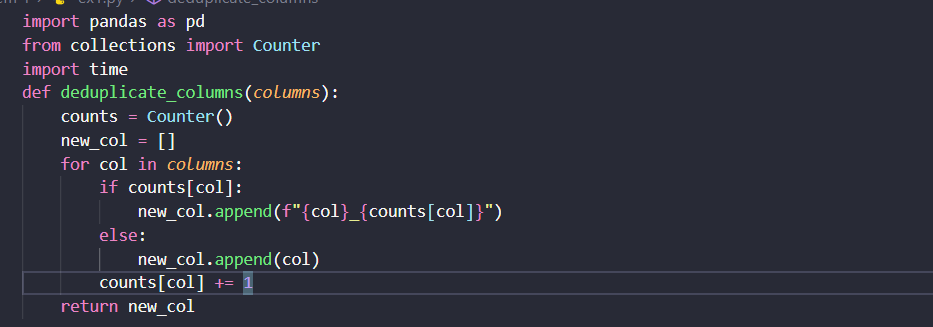
\includegraphics[width=1\textwidth]{img/ham_rename_col.png}
    \end{figure}
    - Sử dụng thư viện collections để đếm số lần xuất hiện của cột.
    - Duyệt qua tất cả các cột có trong dataframe kiểm tra số lần xuất hiện thông qua. counts[col]
    \begin{itemize}
        \item Nếu cột có counts[col] == 0 tức là lần đầu được duyệt -> đẩy vào list new\_col.
        \item Nếu cột có counts[col] != 0 -> đưa vào new\_col với tên mới là \textbf{tên côt + số lần xuất hiện}.
    \end{itemize}
    
\subsubsection{Hàm cài đặt Dataframe}
    - Tạo hàm crawl\_data\_table chuyền vào ba tham số là df(dữ liệu dataframe), list(các cột dữ liệu đề bài yêu cầu), club(tên câu lạc bộ).\\
    \begin{figure}[H]
        \centering
        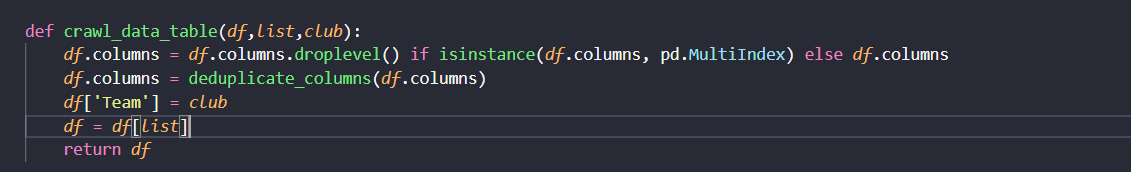
\includegraphics[width=1\textwidth]{img/set_df.png}
    \end{figure}
    - \textbf{\textit{df.columns = df.columns.droplevel() if isinstance(df.columns, pd.MultiIndex) else df.columns}}: câu lệnh xóa bỏ kiểu multiindex của col.
    \begin{itemize}
        \item Kiểm tra xem hàng các cột có phải kiểu multiindex không: \textbf{\textit{isinstance(df.columns, pd.MultiIndex)}}.
        \item Nếu df.columns là kiểu multiindex thì xóa bỏ  \textbf{\textit{df.columns.droplevel()}} không thì giữ nguyên.
    \end{itemize}
    - \textbf{\textit{df.columns = deduplicate\_columns(df.columns)}}: Gọi hàm deduplicate\_columns để đạt lại tên các cột do có các cột bị trùng tên.\\
    - \textbf{\textit{df['Team'] = club}}: Thêm cột Team với giá trị là club.\\
    - \textbf{\textit{df = df[list]}}: Cài đặt lại dataframe lấy các giá trị theo đề bài.

\subsubsection{Hàm tạo Dataframe}
    - Cài đặt hàm trả về một dataframe\\
    \begin{figure}[H]
        \centering
        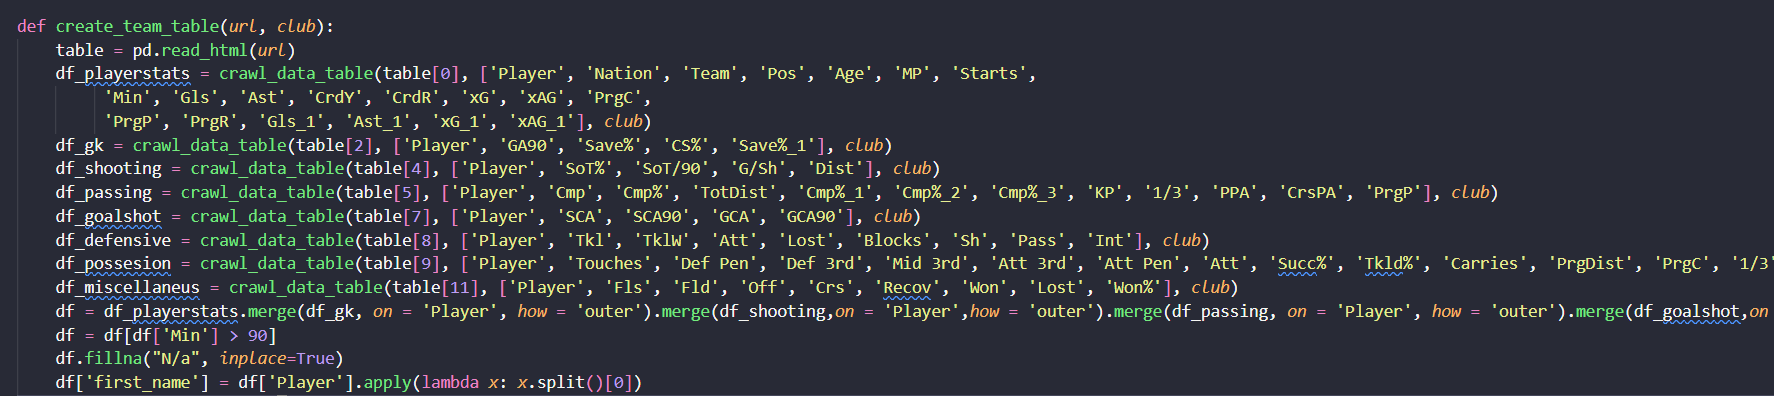
\includegraphics[width=1\textwidth, height=6cm]{img/tao_bang.png}
    \end{figure}
    - Sử dụng hàm \textbf{read\_html()} trong thư viện pandas để đọc các bảng dữ liệu có trong url.\\
    - Khởi tạo các dataframe \textbf{\textit{df\_playerstats, df\_gk, df\_shooting, df\_passing, df\_goalshot, df\_defensive, df\_possesion, df\_miscellaneus}} bàng hàm \textbf{\textit{crawl\_data\_table}} với vị trí bảng tương ứng trong url và các giá trị đề bài yêu cầu cùng tên club.\\
    - Khởi tạo dataframe \textbf{df} là dataframe tổng của các dataframe trên bằng cách \textbf{merge} tất cả các dataframe trên lại dựa vào thuộc tính \textbf{on = 'Player'} (merge các dataframe dựa vào tên cầu thủ) và cách thức \textbf{how = 'outer'} (thêm các giá trị mà dataframe trước không có).\\
    - \textbf{df = df[df['Min] > 90]}: Chỉ lấy các cầu thủ có thời gian trên 90 phút.\\
    - \textbf{df.fillna("N/a", inplace=True)}: Thay thế tất cả các giá trị null bằng 'N/a'.\\
    \begin{figure}[H]
        \centering
        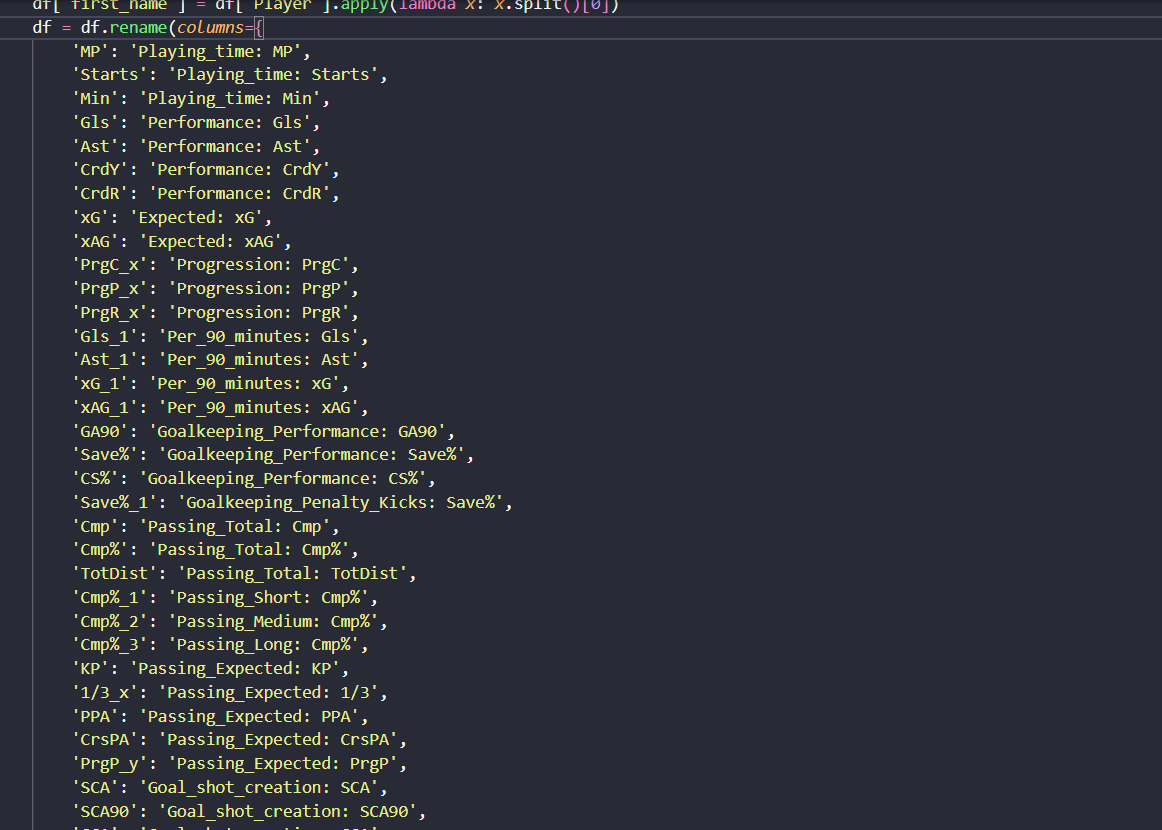
\includegraphics[width=1\linewidth, height=15cm]{img/rename.png}
    \end{figure}
    - Sử dụng hàm \textbf{rename} có sẵn trong thư viện pandas để cài đặt lại tên các cột.\\
    - Tên các cột bằng \textbf{Tên các nhóm chỉ số + tên chỉ số}.\\
    VD: chỉ số \textbf{Gls} trong nhóm chỉ số \textbf{Performance} -> \textbf{Performance: Gls}\\
    - Cuối cùng hàm trả về dataframe hoàn chỉnh.\\

\subsubsection{Viết chương trình trong hàm main}
    \begin{figure}[H]
        \centering
        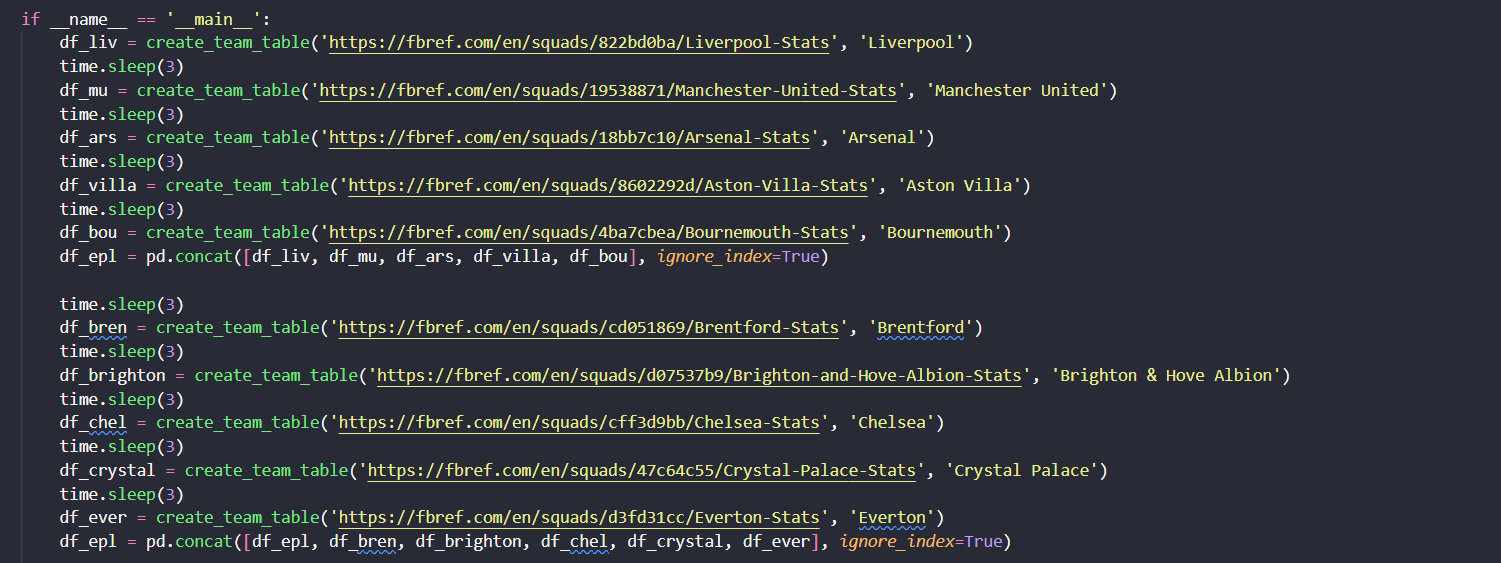
\includegraphics[width=1\linewidth]{img/collect_10_team_first.png}
    \end{figure}
    \begin{figure}[H]
        \centering
        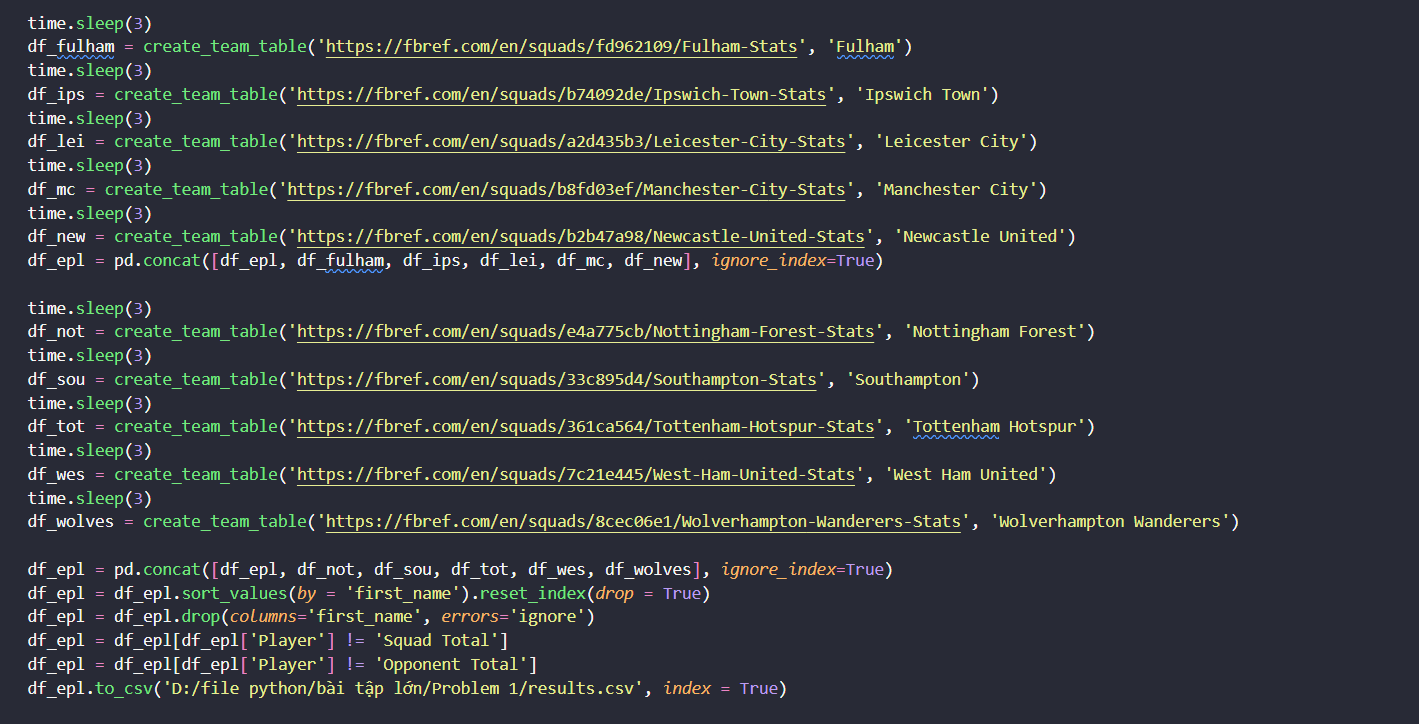
\includegraphics[width=1\linewidth]{img/collect_10_second.png}
    \end{figure}
    - Viết chương trình trong hàm main.\\
    - Sử dụng hàm \textbf{create\_team\_table} để tạo dataframe cho từng đội bóng.\\
    - Giữa mỗi lần lấy dữ liệu của đội bóng thêm \textbf{time.sleep(3)} để tránh bị web chặn.\\
    - Khởi tạo \textbf{\textit{df\_epl}} bằng gộp các dataframe đội bóng bằng hàm \textbf{concat} trong thư viện pandas với \textbf{ignore\_index=True} (khởi tạo lại index cho dataframe sau khi gộp).\\
    - Chia nhỏ lần gửi request (5 đội bóng liên tiếp xong gộp vào với \textbf{df\_epl} luôn để tránh bị web chặn request).\\
    - Sau khi có dữ liệu của tất cả các cầu thủ trong dataframe \textbf{df\_epl} ta thực hiện sắp xếp theo \textbf{first\_name} có reset index sau khi sắp xếp: \textbf{df\_epl = df\_epl.sort\_values(by = 'first\_name')\\.reset\_index(drop = True)}.\\
    - Loại bỏ cột \textbf{first\_name} và các hàng có 'Player' = 'Squad Total' và 'Opponent Total':
    \begin{itemize}
        \item \textbf{df\_epl = df\_epl.drop(columns='first\_name', errors='ignore')}
        \item \textbf{df\_epl = df\_epl[df\_epl['Player'] != 'Squad Total']}
        \item \textbf{df\_epl = df\_epl[df\_epl['Player'] != 'Opponent Total']}
    \end{itemize}
    - Cuối cùng lưu kết quả dataframe hoàn chỉnh vào file 'results.csv' bằng câu lệnh: \\ 
    \textbf{df\_epl.to\_csv('D:/file python/bài tập lớn/Problem 1/results.csv', index = True)}